\appendix
\clearpage
\newpage
\onecolumn

\section{Proof of Corollary~\ref{cor:starc}}\label{A:starc}
\begin{definition}
     A \textit{potential function} is a function $\Phi: \mathcal{S}\xrightarrow{} \mathbb{R}$. Given a discount $\gamma$, $r_1$ and $r_2$ differ by potential shaping if for some potential $\Phi$, we have that $r_2(s,a,s')=r_1(s,a,s')+\gamma\cdot\Phi(s')-\Phi(s)$. 
\end{definition}

\begin{definition}
    Given a transition function $\mathcal{T}$, $r_1$ and $r_2$ differ by \textit{$S'$-redistribution} if $\mathbb{E}_{S' \sim \mathcal{T}(s,a)}[r_2(s,a,s')]=\mathbb{E}_{S' \sim \mathcal{T}(s,a)}[r_1(s,a,s')]$. 
\end{definition}

\begin{definition}
    $r_1$ and $r_2$ differ by positive linear scaling if $r_2(s,a,s')=c \cdot r_1(s,a,s')$ for some positive constant $c$.
\end{definition}
\begin{proof}
    Theorem 2.6 from~\cite{skalse2023misspecification} says that two tasks $\tau_1,\tau_2$ have the same ordering of policies if and only if $r_1$ and $r_2$ differ by potential shaping, positive linear scaling, and $S'$-redistribution. Therefore, if we could find optimal policies for these two tasks separately; they necessarily differ.
    And by forming a policy committee of these two optimal policies, we have $V^{\Pi}_{\tau_1}\ge V^{\pi}_{\tau_1}$, $V^{\Pi}_{\tau_2}\ge V^{\pi}_{\tau_2}$, and $V^{\Pi}_{\tau_1}+V^{\Pi}_{\tau_1} > V^{\pi}_{\tau_1}+ V^{\pi}_{\tau_2}$ for any policy $\pi$.
\end{proof}



%\end{proof}

\section{ Proof of Theorem \ref{thm:NPhard}}\label{A:NP}





\begin{definition}[Gap preserving reduction for a maximization problem]
    %(Gap preservation reduction for a maximisation problem) 
    Assume $\Pi_1$ and $\Pi_2$ are some maximization problems. A gap-preserving reduction from $\Pi_1$ to $\Pi_2$ comes with four parameters (functions) $f_1, \alpha, f_2$ and $\beta$. Given an instance $x$ of $\Pi_1$, the reduction computes in polynomial time an instance $y$ of $\Pi_2$ such that:
$OPT(x) \ge f_1(x) \implies OPT(y) \ge f_2(y)$
and
$OPT(x) < \alpha |x| f_1(x) \implies OPT(y) < \beta |y| f_2(y)$.
\end{definition}

\begin{proof}

Let $G = (V , E)$ be an undirected graph with $5$ vertices and $2$ edges as follows: 

\begin{center}
      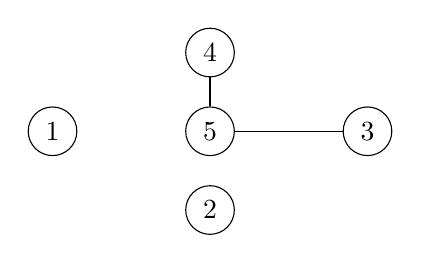
\begin{tikzpicture}
    \foreach \pos/\name in {{(0,1)/1}, {(2,0)/2}, {(4,1)/3}, {(2,2)/4}, {(2,1)/5}}
        \node[circle,draw] (\name) at \pos {$\name$};
    % Define edges
    \foreach \source/\dest in {3/5, 4/5}
        \path (\source) edge (\dest);
\end{tikzpicture}
\end{center}


We create an instance of Max-coverage for a set of $\theta$s in $\mathbb{R}^n$
by filling out their coordinate matrix
$A_{ij}=\begin{cases}
0 & \text{if } i=j\\

    1.5\epsilon & \text{if } i,j \text{ are adjacent} \\
     2.5 \epsilon & \text{if } i,j \text{ are not adjacent}\end{cases}   $ :


\begin{table}[h!]
\centering
 \begin{tabular}{c|ccccc}
         dim & $\theta_1$ & $\theta_2$ & $\theta_3$ & $\theta_4$ & $\theta_5$\\ \hline

    $1$&     0 & 2.5& 2.5 & 2.5 & 2.5 \\
    $2$&     2.5 & 0& 2.5 & 2.5 & 2.5 \\
$3$&     2.5 & 2.5& 0 & 2.5 & 1.5 \\
$4$&     2.5 & 2.5& 2.5 & 0 & 1.5 \\
$5$&     2.5 & 2.5& 1.5 & 1.5 & 0 \\
    \end{tabular}
   
    \label{tab:my_label}
\end{table}



Let $\theta_1=[0,2.5,2.5,2.5,2.5]$,
$\theta_2=[2.5,0,2.5,2.5,2.5]$,
$\theta_3=[2.5,2.5,0,2.5,1.5]$,
$\theta_4=[2.5,2.5,2.5,0,2.5]$,
$\theta_5=[2.5,2.5,1.5,1.5,0].$




Projected onto the fifth axis, our thetas look like:




\begin{center}
    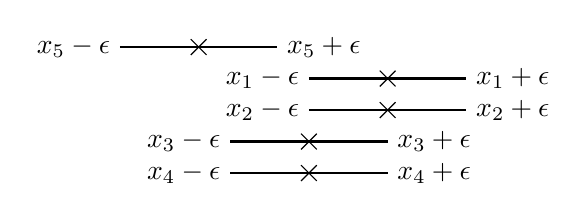
\begin{tikzpicture} [scale=2]
 
% First line segment
\draw[thick] (0,0) coordinate (A) -- (1,0) coordinate (B);
\draw (A) node[left] {$x_4-\epsilon$};
\draw (B) node[right] {$x_4+\epsilon$};

{%
    \draw (0.5-0.05,-0.05) -- (0.5+0.05,0.05);
    \draw (0.5-0.05,0.05) -- (0.5+0.05,-0.05);
}

% Second line segment
\draw[thick] (0,0.2) coordinate (C)-- (1,0.2)coordinate (D);
\draw (C) node[left] {$ x_3-\epsilon$};
\draw (D) node[right] {$x_3+\epsilon$};

{%
    \draw (0.5-0.05,0.2-0.05) -- (0.5+0.05,0.2+0.05);
    \draw (0.5-0.05,0.2+0.05) -- (0.5+0.05,0.2-0.05);
}

% Third line segment
\draw[thick] (0.5,0.4) coordinate (E) -- (1.5,0.4) coordinate (F);
\draw (E) node[left] {$x_2-\epsilon$};
\draw (F) node[right] {$x_2+\epsilon$};
{%
    \draw (1-0.05,0.4-0.05) -- (1+0.05,0.4+0.05);
    \draw (1-0.05,0.4+0.05) -- (1+0.05,0.4-0.05);
}



% Third line segment
\draw[thick] (0.5,0.6) coordinate (E) -- (1.5,0.6) coordinate (F);
\draw (E) node[left] {$ x_1-\epsilon$};
\draw (F) node[right] {$x_1+\epsilon$};
{%
    \draw (1-0.05,0.6-0.05) -- (1+0.05,0.6+0.05);
    \draw (1-0.05,0.6+0.05) -- (1+0.05,0.6-0.05);
}


% Fourth line segment
\draw[thick] (-0.7,0.8) coordinate (G) -- (0.3,0.8) coordinate (H);
\draw (G) node[left] {$ x_5-\epsilon$};
\draw (H) node[right] {$x_5+\epsilon$};
{%
    \draw (-0.2-0.05,0.8-0.05) -- (-0.2+0.05,0.8+0.05);
    \draw (-0.2-0.05,0.8+0.05) -- (-0.2+0.05,0.8-0.05);
}


\end{tikzpicture}
\end{center}

And similarly, onto the third axis:


\begin{center}
    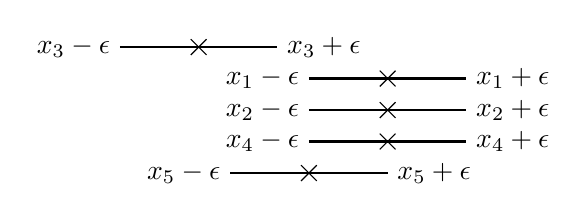
\begin{tikzpicture} [scale=2]
 
% First line segment
\draw[thick] (0,0) coordinate (A) -- (1,0) coordinate (B);
\draw (A) node[left] {$x_5-\epsilon$};
\draw (B) node[right] {$x_5+\epsilon$};

{%
    \draw (0.5-0.05,-0.05) -- (0.5+0.05,0.05);
    \draw (0.5-0.05,0.05) -- (0.5+0.05,-0.05);
}

% Second line segment
\draw[thick] (0.5,0.2) coordinate (C)-- (1.5,0.2)coordinate (D);
\draw (C) node[left] {$ x_4-\epsilon$};
\draw (D) node[right] {$x_4+\epsilon$};

{%
    \draw (1-0.05,0.2-0.05) -- (1+0.05,0.2+0.05);
    \draw (1-0.05,0.2+0.05) -- (1+0.05,0.2-0.05);
}

% Third line segment
\draw[thick] (0.5,0.4) coordinate (E) -- (1.5,0.4) coordinate (F);
\draw (E) node[left] {$x_2-\epsilon$};
\draw (F) node[right] {$x_2+\epsilon$};
{%
    \draw (1-0.05,0.4-0.05) -- (1+0.05,0.4+0.05);
    \draw (1-0.05,0.4+0.05) -- (1+0.05,0.4-0.05);
}



% Third line segment
\draw[thick] (0.5,0.6) coordinate (E) -- (1.5,0.6) coordinate (F);
\draw (E) node[left] {$ x_1-\epsilon$};
\draw (F) node[right] {$x_1+\epsilon$};
{%
    \draw (1-0.05,0.6-0.05) -- (1+0.05,0.6+0.05);
    \draw (1-0.05,0.6+0.05) -- (1+0.05,0.6-0.05);
}


% Fourth line segment
\draw[thick] (-0.7,0.8) coordinate (G) -- (0.3,0.8) coordinate (H);
\draw (G) node[left] {$ x_3-\epsilon$};
\draw (H) node[right] {$x_3+\epsilon$};
{%
    \draw (-0.2-0.05,0.8-0.05) -- (-0.2+0.05,0.8+0.05);
    \draw (-0.2-0.05,0.8+0.05) -- (-0.2+0.05,0.8-0.05);
}


\end{tikzpicture}
\end{center}







We claim that we have constructed a gap-preserving reduction for any $t>0$
$$OPT(A) = n \implies OPT(B) = n $$
$$OPT(A) < n^{1-t} \implies OPT(B) < n^{1-t}.$$


To begin with, if the Max-Clique instance consists of a complete graph, then the $\theta$s we created have coordinates equal to $1.5\epsilon
$ everywhere except $i$-th coordinate, which is zero. So they can all be covered by one $\Tilde{\theta}=[0.7\epsilon,0.7\epsilon,\dots,0.7\epsilon]$, the coverage size is $n$. Therefore, the first implication is true.

Then for the second statement, we argue with the contrapositive: assume that one of the maximum coverage sets is $S=\{i_1,\dots,i_k\}$ and $k\ge n^{1-t}$. We have to prove that the maximum clique has size greater than or equal to $k\ge n^{1-t}$. 

Specifically, we prove that the vertices corresponding to the elements from $S$ form a clique.

If $\theta_i,\theta_j$ are from the set $S$, then they should be covered on each dimension since the $||\theta_i-\theta_j||_\infty= \max |\theta_i^d-\theta_j^d| \le \epsilon.$ So $\theta_i,\theta_j$ have to be adjacent, because otherwise their corresponding coordinates on the $i$-th and $j$-th dimension are more than $\epsilon$ away. 
For example, we have theta $\theta_3^3=0$ and $\theta_5^5=0$, so $\theta_5^3$ and  $\theta_5^3$ must be $1.5\epsilon$ rather than $2.5\epsilon$, which indicates that $3, 5$ are neighbors in the graph.

Therefore, the points in $S$ correspond to 
a clique of size $k \ge n^{1-t}$
%the maximum-clique 
in the graph.  
Thus, if the graph $G$ has a clique of size less than $n^{1-t}$, then the maximum coverage set has size less than $n^{1-t}$.
%Therefore, the reduction presented above is a gap-preserving reduction. A gap-preserving reduction from $A$ to $B$ with the above parameters implies that if the problem $A$ cannot have a polynomial-time $\alpha$-approximation, then the problem $B$ cannot have a polynomial-time $\beta$-approximation.
\end{proof}

\section{Pseudocode of Greedy Intersection Algorithm} \label{S:code}

The full pseudocode for the \emph{Greedy Intersection Algorithm (GIA)} algorithm is provided as Algorithm~\ref{alg:greedy_intersection}.

\begin{algorithm}[h]
    \caption{Greedy Intersection}
    \label{alg:greedy_intersection}
    \textbf{Input}: $T = \{\theta_i\}_{i=1}^N$, $\epsilon > 0$, $K \ge 1$ \\
    \textbf{Output}: Parameter cover $C$
    \begin{algorithmic}[1]
    \STATE $C \gets []$
        \FOR{$round\ k$ = $1$ to $K$}
            \FOR{$dimension\ m$ = $1$ to $d$}
                \STATE Sort $T$ in ascending order based on their $m$-th coordinates
                \STATE $lists_m \gets []$
                \FOR{$indiviual\ i = 2$ to $N$}
                    \STATE $S_i \gets [\theta_i]$
                    \FOR{$j = i-1$ to $1$}
                        \IF{$\theta_i$'s $m$-th coordinate $< \theta_j$'s $m$-th coordinate $+2\epsilon$}
                            \STATE Add $\theta_j$ to $S_i$
                        \ELSE
                            \IF{ $lists_m[-1] \subseteq S_{i}$ }
                                \STATE $lists_m[-1] \gets S_{i}$ 
                            \ELSE
                                \STATE Add $S_{i}$ to $lists_m$
                            \ENDIF
                            \STATE \textbf{break}
                        \ENDIF
                    \ENDFOR
                \ENDFOR
            \ENDFOR

            \STATE $S^{1*},\dots, S^{m*} \gets  \text{argmax}_{S^1\in lists_1,\dots, S^m\in lists_m} |S^1\cap \dots \cap S^m|$
             \STATE $covered \gets S^{1*}\cap \dots \cap S^{m*}$
              \STATE $\hat{\theta}_k \gets $ average of the $covered$
            \STATE $T \gets T - covered$
            \STATE $C$.adds($\hat{\theta}_k$)
        \ENDFOR
        \STATE \textbf{return} $C$
    \end{algorithmic}
\end{algorithm}



\section{ Proof of Theorem \ref{thm:greedy_gaurantee}} \label{A:greedy_gaurantee}
Based on the proof of maxmizing monotone submodular functions by \cite{nemhauser1978analysis}.





   


%Suppose all $\theta$s are drawn i.i.d. from the same distribution $\Gamma$. Let $\Pi^*$ be the coverage area of the optimal committee. And let $OPT$ denote the maximal probability of a $\theta$ being covered by a committee of fixed size $K$, i.e., $OPT=\Pr_{\theta \sim \Gamma}[\theta \in \Pi^*].$
    %Consider algorithm \ref{alg:greedy_intersection}, let $A_i$ denote the region covered by the representative selected on the $i$-th iteration.  And denote $C_i$ as the set of $\theta$s from the dataset that are covered after $i$-th iteration.  With probability at least 
    %$1-\delta_1 \ge 
    %$\frac{1+\sqrt[\leftroot{-2}\uproot{2}4]{1-\delta}}{2}$, the probability of the new $\theta$ falls into $A_i$, but not $\bigcup_{j=1}^{i-1} A_j$ is greater than $OPT-(\frac{|C_{i-1}|}{N}+\epsilon)$.










%With $N$ greater than $\frac{9\log(\frac{1-\sqrt[\leftroot{-2}\uproot{2}4]{1-\delta}}{2})}{-2\epsilon^2}$, whose complexity is in $\mathcal{O}(\frac{1}{\epsilon^2}\log\delta)$, we can make sure that $\delta_1 \le \frac{1-\sqrt[\leftroot{-2}\uproot{2}4]{1-\delta}}{2}$, which be needed in later steps.


 


\begin{lemma}\label{lm:pf4}Suppose $1-\delta^*(K)$ is the optimal $(\epsilon,1-\delta)$-parameter-cover of $\Gamma$ achievable with fixed $K$. With probability at least $1-\alpha$ ,
    the probability of $\theta$ from $\Gamma$ getting covered by the first $i$ representatives generated by Algorithm \ref{alg:greedy_intersection} is greater than $\frac{1-\delta^*(K)-K\beta}{K}\sum_{j=0}^{i-1}(1-1/K)^j.$
\end{lemma} 
\begin{proof} We will prove the lemma through induction. We begin by defining the coverage region of each of the $K$ committee member in the optimal parameter-cover as $S^*_i.$ Furthermore, let $\Pi^*$ denote the region covered by this optimal parameter-cover. Thus, $\Pi^*=\bigcup S_i^*.$ Next, let $A_i$ denote the region covered by the representative selected on the $i$-th iteration.  And let  $C_{i}$ denote the set of $\theta$s from the dataset $T$ that are covered after $i$-th iteration.


First of all, we want to show  at $i=1$, the probability for $\theta \sim \Gamma$ getting covered is greater than
$\frac{1-\delta^*(K)-K\beta}{K}\sum_{j=0}^{0}(1-1/K)^0=\frac{1-\delta^*(K)-K\beta}{K}.$

By Hoeffding's theorem, $\Pr_{\theta \sim \Gamma}[\mathbb{E}_{\theta \sim \Gamma}[\mathbf{1}(\theta\in \bigcup_{j=1}^{i-1} A_j)]- \frac{\sum_i \mathbf{1}(\theta_i\in \bigcup_{j=1}^{i-1} A_j)}{N}  ) \ge \frac{\beta}{3}] \le \exp(-2N\beta^2/9)=\frac{\alpha}{5}.$ Hence, with probability at least $1-\frac{\alpha}{5}$,
 $\Pr_{\theta \sim \Gamma} [\theta \in \bigcup_{j=1}^{i-1} A_j] =\mathbb{E}_{\theta \sim \Gamma}[\mathbf{1}(\theta\in \bigcup_{j=1}^{i-1} A_j)] \le \frac{\sum_i \mathbf{1}(\theta_i\in \bigcup_{j=1}^{i-1} A_j)}{N}+\frac{\beta}{3} =\frac{|C_{i-1}|}{N}+\frac{\beta}{3}.$ 
 %For convenience's sake, we take $\alpha_1$ as the shorthand for $\frac{1-\sqrt[\leftroot{-2}\uproot{2}4]{1-\alpha}}{2}.$

 
    Now the union bound first gives that $\Pr_{\theta \sim \Gamma}[ \theta \in \Pi^* \land \theta \notin \bigcup_{j=1}^{i-1} A_j ]\ge \Pr_{\theta \sim \Gamma}[ \theta \in \Pi^*] - \Pr_{\theta \sim \Gamma} [\theta \in \bigcup_{j=1}^{i-1} A_j]=1-\delta^*(K) - \Pr_{\theta \sim \Gamma} [\theta \in \bigcup_{j=1}^{i-1} A_j].$ Applying union bound again, we obtain that with probability at least $1-\alpha_1$,
    $\sum_{i=1}^K\Pr_{\theta \sim \Gamma}[\theta \in S_i^* \land \theta \notin \bigcup_{j=1}^{i-1} A_j] \ge \Pr_{\theta \sim \Gamma}[\theta \in \Pi^* \land \theta \notin \bigcup_{j=1}^{i-1} A_j] \ge 1-\delta^*(K)-(\frac{|C_{i-1}|}{N}+\frac{\beta}{3}) $.
    Hence, $\max_{i\in [K]} \Pr_{\theta \sim \Gamma}[\theta \in S_i^* \land \theta \notin \bigcup_{j=1}^{i-1} A_j] \ge \frac{ 1-\delta^*(K)-(\frac{|C_{i-1}|}{N}+\frac{\beta}{3})}{K}.$ Let us call this maximising $S_i^*$ 
    $\hat{S}.$


    
 %We can conclude that  with probability at least $\frac{1+\sqrt[\leftroot{-2}\uproot{2}4]{1-\alpha}}{2}$, $\Pr_{\theta \sim \Gamma}[ \theta \in \Pi^* \land \theta \notin \bigcup_{j=1}^{i-1} A_j ]\ge 1-\delta^*(K)-(\frac{|C_{i-1}|}{N}+\frac{\beta}{3}).$




    
According to our Algorithm~\ref{alg:greedy_intersection}, $A_i$ covers the most $\theta$s from $T$ that were not covered in the previous rounds by $\bigcup_{j=1}^{i-1} A_j$. In particular, $|C_i|-|C_{i-1}|$ is greater or equal to the number of $\theta$s from $T$ covered in $\hat{S}$ but not $\bigcup_{j=1}^{i-1} A_j$. Let us denote the latter as $s_1$, and the former as $s_2,$ then $s_1-s_2 \le 0.$





Hoeffding's theorem gives us $\Pr_{\theta \sim \Gamma}(\mathbb{E}_{\theta \sim \Gamma}[\mathbf{1}[\theta \in \hat{S} \land \theta \notin \bigcup_{j=1}^{i-1} A_j]]-s_1/N) \ge \frac{\beta}{6}) \le (\frac{\alpha}{5})^4$ and $\Pr_{\theta \sim \Gamma}(s_2/N- \mathbb{E}_{\theta \sim \Gamma}[\mathbf{1}[\theta \in A_i \land \theta \notin \bigcup_{j=1}^{i-1} A_j]] \ge \frac{\beta}{6}) \le (\frac{\alpha}{5})^4$. Hence
with probability at least $1-2(\frac{\alpha}{5})^4$, 
$\mathbb{E}_{\theta \sim \Gamma}[\mathbf{1}[\theta \in \hat{S} \land \theta \notin \bigcup_{j=1}^{i-1} A_j]]-\mathbb{E}_{\theta \sim \Gamma}[\mathbf{1}[\theta \in A_i \land \theta \notin \bigcup_{j=1}^{i-1} A_j]]=(\mathbb{E}_{\theta \sim \Gamma}[\mathbf{1}[\theta \in \hat{S} \land \theta \notin \bigcup_{j=1}^{i-1} A_j]]-s_1/N)+ (s_1-s_2)/N+ (s_2/N-\mathbb{E}_{\theta \sim \Gamma}[\mathbf{1}[\theta \in A_i \land \theta \notin \bigcup_{j=1}^{i-1} A_j]]\le\frac{\beta}{6}+\frac{\beta}{6}= \frac{\beta}{3}.$

Applying the result we obtained at the beginning of the proof, we have with probability at least $1-\frac{\alpha}{5}-2(\frac{\alpha}{5})^4$, 


\begin{align}
     &\Pr_{\theta \sim \Gamma}[\theta \in A_i \land \theta \notin \bigcup_{j=1}^{i-1} A_j] \nonumber \\
     \ge& \Pr_{\theta \sim \Gamma}[\theta \in \hat{S}\land \theta \notin \bigcup_{j=1}^{i-1} A_j] -\frac{\beta}{3} \nonumber
     \\ \ge& \frac{ 1-\delta^*(K)-(\frac{|C_{i-1}|}{N}+\frac{\beta}{3})}{K} -\frac{\beta}{3} \label{step1}.
\end{align}


%with probability at least $(1-\exp(4\log(1-\frac{1-\sqrt[\leftroot{-2}\uproot{2}4]{1-\alpha}}{2})))^2$, $\mathbb{E}(s_1)-\mathbb{E}(s_2) = (\mathbb{E}(s_1)-s_1/N)+ (s_1-s_2)/N+ (s_2/N-\mathbb{E}(s_2)) \le \frac{\beta}{6}+\frac{\beta}{6}= \frac{\beta}{3}.$ 



%Suppose $S_2-S_1\ge\beta N/9.$ Then Hoeffding gives us, with probability at least $1-\delta \le (1-\delta_1)^2$, $\Pr_{\theta \sim \Gamma}[\theta \in A_i \land \theta \notin \bigcup_{j=1}^{i-1} A_j] \ge  \Pr_{\theta \sim \Gamma}[\theta \in \hat{S}\land \theta \notin \bigcup_{j=1}^{i-1} A_j]  $, since with probability $1-\delta_1$ respectively,$\Pr_{\theta \sim \Gamma}[\theta \in A_i \land \theta \notin \bigcup_{j=1}^{i-1} A_j]\ge |S_2/N|-\beta/18$ and $\Pr_{\theta \sim \Gamma}[\theta \in S_i^* \land \theta \notin \bigcup_{j=1}^{i-1} A_j]\le |S_1/N|+\beta/18 $, leading to $ \Pr_{\theta \sim \Gamma}[\theta \in S_i^* \land \theta \notin \bigcup_{j=1}^{i-1} A_j]\le |S_2/N|-\beta/9+\beta/18 \le \Pr_{\theta \sim \Gamma}[\theta \in A_i \land \theta \notin \bigcup_{j=1}^{i-1} A_j]. $

%Alternatively, if $0 \le S_2-S_1 \le \beta N/9,$ then with probability at least $1-\delta$,  $\Pr_{\theta \sim \Gamma}[\theta \in A_i \land \theta \notin \bigcup_{j=1}^{i-1} A_j] \ge \Pr_{\theta \sim \Gamma}[\theta \in \hat{S} \land \theta \notin \bigcup_{j=1}^{i-1} A_j] -\frac{\beta}{3}  $. 



Since nothing is covered before the first iteration, we can use step (\ref{step1}) with $|C_{0}|=0$ to prove the base condition for the claim.
Because $K\ge1$,  we have $\frac{ 1-\delta^*(K)-\frac{\beta}{3}}{K} -\frac{\beta}{3} =\frac{ 1-\delta^*(K)-\frac{(1+K)\beta/3}{K}}{K} \ge \frac{1-\delta^*(K)-K\beta}{K}.$


The induction hypothesis is that for all $i\le K-1$,
we have $ \Pr_{\theta \sim \Gamma}[\theta \in \bigcup_{j=1}^{i} A_j] \ge \frac{1-\delta^*(K)-K\beta}{K} \sum_{j=0}^{i}(1-1/K)^j.$

By Hoeffding, $\Pr_{\theta \sim \Gamma}[|\Pr_{\theta \sim \Gamma}[\theta \in \bigcup_{j=1}^{i-1} A_j]- \frac{|C_{i-1}|}{N}| \ge \beta/3 ] \le 2\exp(-2N\beta^2/9).$ In other words, with probability at least $1-2\frac{\alpha}{5}$, $\Pr_{\theta \sim \Gamma}[\theta \in \bigcup_{j=1}^{i-1} A_j]\ge \frac{|C_{i-1}|}{N}-\beta/3 $ and $ \frac{|C_{i-1}|}{N} \ge \Pr_{\theta \sim \Gamma}[\theta \in \bigcup_{j=1}^{i-1} A_j]- \beta/3.$




%and $\Pr_{\theta \sim \Gamma}[\Pr_{\theta \sim \Gamma}[\theta \in \bigcup_{j=1}^{i-1} A_j] \ge \frac{|C_{i-1}|}{N}+ \beta/3]\le $ respectively.

Then at the step $i=K$, since for $\frac{\alpha}{5}\in (0,1), (\frac{\alpha}{5})^4 <\frac{\alpha}{5}$, we have with probability at least $1-2\frac{\alpha}{5}-\frac{\alpha}{5}-2(\frac{\alpha}{5})^4 \ge 1-5 \frac{\alpha}{5}=1-\alpha$,
\begin{align*}
    &\Pr_{\theta \sim \Gamma}[\theta \in \bigcup_{j=1}^{i} A_j]\\
    =&\Pr_{\theta \sim \Gamma}[\theta \in \bigcup_{j=1}^{i-1} A_j]+   \Pr_{\theta \sim \Gamma}[\theta \in A_i \land \theta \notin \bigcup_{j=1}^{i-1} A_j]  \\
    \ge &\frac{|C_{i-1}|}{N}-\frac{\beta}{3}             +\frac{ 1-\delta^*(K)-(\frac{|C_{i-1}|}{N}+\beta/3)}{K} -\frac{\beta}{3}  \\
    = &\frac{1-\delta^*(K)}{K}+(1-1/K) \frac{|C_{i-1}|}{N} - \frac{(2K+1)\beta}{3K}\\
    \ge &\frac{1-\delta^*(K)}{K}+(1-1/K) (\Pr_{\theta \sim \Gamma}[\theta \in \bigcup_{j=1}^{i-1} A_j]-\beta/3)- \frac{(2K+1)\beta}{3K} \\
    \ge &\frac{1-\delta^*(K)}{K}+(1-1/K)\bigl(\frac{1-\delta^*(K)-K\beta}{K}  \sum_{j=0}^{i-1}(1-1/K)^j\bigr)-(1-1/K)\beta/3- \frac{(2K+1)\beta}{3K} \\
    =&\frac{1-\delta^*(K)}{K}-\frac{(2K+1+K-1)\beta}{3K} +\frac{1-\delta^*(K)-K\beta}{K} \sum_{j=1}^{i}(1-1/K)^j\\
   = &\frac{1-\delta^*(K)-K\beta}{K} \sum_{j=0}^{i}(1-1/K)^j
\end{align*}
\end{proof}



\begin{proof}[Proof of Theorem \ref{thm:greedy_gaurantee}]
We can directly apply lemma~\ref{lm:pf4} to $i=K$. Call the region defined by the cover generated by Algorithm~\ref{alg:greedy_intersection} $\Pi_K=\bigcup_{j=1}^{K} A_j.$ Using the inequality $(1-1/K)^K \ge 1-1/e$ for all $K \ge 0$, we have

\begin{align*}
   \Pr_{\theta \sim \Gamma}[\theta \in \Pi_K] 
   \ge&
\frac{1-\delta^*(K)-K\beta}{K} \sum_{j=0}^{K}(1-1/K)^j\\
=&
\frac{1-\delta^*(K)-K\beta}{K} \frac{1-(1-1/K)^K}{1-(1-1/K)}\\
=&
(1-\delta^*(K)-K\beta)({1-(1-1/K)^K})\\
\ge& (1-1/e)(1-\delta^*(K)-K\beta).
\end{align*}




%After drawing $n$ samples $z_1,z_2,\dots$, we proceed the greedy coverage procedure on the set.By Hoeffding's theorem, $\Pr[\frac{\sum_i \mathbbm{1}(z_i \text{is covered by} \Pi)}{n}  -\mathbb{E}(\mathbbm{1}(z \text{ is covered by} \Pi)) \ge \beta] \le 2\exp(-2n\beta^2)=\delta.$And $\frac{\sum_i \mathbbm{1}(z_i \text{is covered by} \Pi)}{n}$ is the $(1-\frac{1}{e})\Pr_{OPT}$
\end{proof}


\iffalse
\section{Proof of Theorem \ref{thm:set_cover}}

\begin{theorem}\label{thm:set_cover}
Suppose $T$ contains $n \ge \frac{8|K^*(\epsilon,\delta)|^2\log({2/\alpha})}{\beta^2}$ i.i.d.~samples from $\Gamma$ and a finite $(\epsilon,1-\delta)$-parameter cover of $\Gamma$ exists. Let $K^*(\epsilon,\delta)$ be the minimal $(\epsilon,1-\delta)$-parameter cover of $\Gamma.$ Then with probability at least $1-\alpha$,
the $GI(\delta)$ is a $(\epsilon,1-\delta-\beta)-$parameter-cover of $\Gamma$ with size at most $\ln(\beta)|K^*(\epsilon,\delta)|.$
%Under sample complexity $\mathcal{O}(\frac{1}{\epsilon}\log\delta)$, with probability $1-\delta$,  a task from the same distribution can be ($1-\epsilon$) covered under a policy committee of size $(1+\ln(x))$ of the optimal number.
\end{theorem}

\begin{proof}[Proof of Theorem \ref{thm:set_cover}]

%Suppose it is finite. $OPT = min | \Pi| $ s.t. $\Pr_{\theta \sim \Gamma}[\theta \in \Pi]=1$



Let us denote the size of the optimal solution $K^*(\epsilon,\delta)$ as $OPT$
%,the covered region by each committee member as $S_i^*$, and the total region covered by $K^*(\epsilon,\delta)$ as $\Pi^*$. Thus, $\Pi^*=\bigcup_{i=1}^{OPT} S_i^*.$
Further, let $N_{i-1}$ be the region still uncovered after the $i-1$th iteration. Then there is also a $(\epsilon,1-\delta)$-parameter-cover with size at most $OPT$ for  $\theta \sim \Gamma, \theta \in N_{i-1}$ since $N_{i-1} \subset N_0$. Let us denote the region covered by each of this parameter-cover as $S_i'$ and the total region covered  by the cover as $\Pi'.$Then by the union bound, $\Pr_{\theta \sim \Gamma}[\theta \in N_{i-1}] -\delta\le \Pr_{\theta \sim \Gamma, \theta \in N_{i-1}}[\theta \in \Pi' ] \le \sum_{j=1}^{OPT}\Pr_{\theta \sim \Gamma, \theta \in N_{i-1}}[\theta \in S'_j] .$

%Then the region could be covered by at most $OPT$ sets since the optimal solution covers the $\Gamma$. And at least one of the set 


Hence at least one $S_j'$ satisfies that $\Pr_{\theta \sim \Gamma, \theta \in N_{i-1}}[\theta \in S'_j ] \ge \frac{\Pr_{\theta \sim \Gamma}[\theta \in N_{i-1}] -\delta}{OPT}$. Let us call it $\hat{S'}.$

Because our algorithm~\ref{alg:greedy_intersection} is completely greedy on the $n$ tasks from $T$, 
the number of samples covered at the $i$-th step is greater than the number of samples covered by $\hat{S'}.$

Let us denote the samples covered at the $i$-th step as $A_i$ and  the samples that could be covered by  $\hat{S'}$ in $N_{i-1}$ as $B_i.$ And the number of samples in $N_{i-1}$ as $n_{i-1}$.

By Hoeffding's theorem, $\Pr_{\theta \sim \Gamma}[[|A_i|/n_{i-1}] \le \mathbb{E}_{\theta \sim \Gamma,\theta \in N_i}[\mathbf{1}[\theta \in A_i]]-\frac{\beta}{4OPT}] \le \exp(-N\beta^2/2)\le \alpha/2$.
And  $\Pr_{\theta \sim \Gamma}[  \mathbb{E}_{\theta \sim \Gamma,\theta \in N_i}[\mathbf{1}[\theta \in \hat{S'}]] \ge |B_i|/n_{i-1} + \frac{\beta}{4OPT}] \le \exp(-N\beta^2/2)\le \alpha/2.$ Hence with probability at least $1-\alpha$  
$\Pr [\theta \in A_i] \ge \Pr [\theta \in \Hat{S}']-\frac{\beta}{2OPT}.$




And the probability of $\theta \sim \Gamma$ still not getting covered after the $i$-th step is 
$\Pr_{\theta \sim \Gamma}[\theta \in N_i]= \Pr_{\theta \sim \Gamma}[\theta \in N_{i-1}] -  \Pr_{\theta \sim \Gamma,\theta \in N_{i}}[\theta \in A_i]\le \Pr_{\theta \sim \Gamma}[\theta \in N_{i-1}] -(\Pr [\theta \in \Hat{S}']-\frac{\beta}{2OPT})\le \Pr_{\theta \sim \Gamma}[\theta \in N_{i-1}] -\frac{\Pr_{\theta \sim \Gamma}[\theta \in N_{i-1}] -\delta}{OPT} +\frac{\beta}{2OPT}.$




%\frac{\Pr[\theta \in N_{i-1}]}{OPT}$since    $\sum_{j=1}^{OPT} \Pr[\theta \in \Pi_j]=1.$


%After step $i$, the probability still not covered is  $\Pr [\theta \in N_i] =   \Pr [\theta \in N_{i-1}] - \Pr [\theta \in A_i]   \le   \Pr [\theta \in N_{i-1}] - (\Pr [\theta \in \Pi_i]-\frac{\beta}{2}\le (1-\frac{1}{OPT}) \Pr [\theta \in N_{i-1}] + \frac{\beta}{2}$ by greedy step $A_i$ will covered the most points $\Pr [\theta \in A_i] \ge \Pr [\theta \in \Pi_i]-\frac{\beta}{2}$ And by Hoeffding with high probability $1-\delta$, $|A_i|/|n_{i-1}| \ge |P_i|/|n_{i-1}|$

Since nothing is covered before the first iteration, $\Pr_{\theta \sim \Gamma} [\theta \in N_0]=1$. By recursion we have 
$\Pr_{\theta \sim \Gamma} [\theta \in N_i] \le (1 -\frac{1}{OPT})^i + \sum(1-\frac{1}{OPT})^i (\frac{\beta}{2OPT}+\frac{\delta}{OPT}).$ 

Consider $i= OPT\ln\frac{2}{\beta}$, because $1-x\le \exp(-x)$ for any $x>0$,
we have 
$\Pr [\theta \in N_i] \le \exp(-\frac{1}{OPT}OPT\ln\frac{2}{\beta}) + (\frac{\beta}{2OPT}+\frac{\delta}{OPT})\frac{1-(1-\frac{1}{OPT})^{OPT\ln\frac{1}{\beta}}}{1-(1-\frac{1}{OPT})} 
\le \frac{\beta}{2}+(\frac{\beta}{2OPT}+\frac{\delta}{OPT}) \frac{1}{1-(1-\frac{1}{OPT})}=\delta +\beta.$


%$(1-\frac{1}{OPT})^i + \sum(1-\frac{1}{OPT})^i \frac{\beta}{2}$$\le (\exp(-\frac{1}{OPT}))^{OPT\ln\frac{2}{\beta}} + \frac{\beta}{2} \cdot \frac{1-(1-\frac{1}{OPT})^{OPT\ln\frac{1}{OPT}}}{1-(1-\frac{1}{OPT})}$

%Let us just denote $OPT$ as $X$ for now.

%$(\exp(-\frac{1}{X}))^{X\ln\frac{2}{\beta}} +\frac{\beta}{2} \cdot \frac{1-(1-\frac{1}{X})^{X\ln\frac{1}{\frac{\beta}{2}}}}{1-(1-\frac{1}{X})}\le \frac{\epsilon}{2} + X \frac{\epsilon}{2}  - X \frac{\epsilon}{2}^2 \le 2\frac{\epsilon}{2}=\epsilon $








%$n_i \le (1-\frac{1}{OPT})^i N.$Consider $i=OPT\ln\frac{N}{OPT},$ $n_i\le (1-\frac{1}{OPT})^{OPT\ln\frac{N}{OPT}}N \le \exp(-\ln\frac{N}{OPT})\cdot N \le \frac{N}{OPT}\cdot N= OPT.$ Hence the remaining at most $OPT$ thetas can be covered by at most $OPT$ sets. The total number of set required with our algorithm is $OPT(1+\ln\frac{N}{OPT}).$ The approximation ratio $1+\ln\frac{N}{OPT}$ is in $\mathcal{O}(\log N)$






\end{proof}
\fi

\section{Proof of Theorem \ref{thm:softmax}}
\label{A:softmax}
\begin{proof}
Let us call the optimal solutions set to \eqref{E:optK} $A_1$, and the optimal solutions set to \eqref{E:relaxK} $A_2$.  

  
We first show $A_1\subset A_2$. Pick any $\{\theta_1,\dots,\theta_K\}\in A_1$. Due to the premise, for each $i$, since $ \min_{k \in [K]}    \|\theta_k-\theta_i\|_\infty - \epsilon \le 0$ ,  there exists $\theta_{k^*}$ such that $ \|\theta_{k^*}-\theta_i\|_\infty - \epsilon \le 0$.
Thus, 
we can have $\alpha_{k^*}(i)=1$, and $\alpha_{k}(i)=0 $ for all the other $k \ne k^*$. 
Then 
$\mathbf{ReLU}\left(\left\{\sum_{k \in [K]} \mathrm{softmax}_k(\alpha_{i})\|\theta_{k}-\theta_i\|_\infty\right\} -\epsilon\right)=\mathbf{ReLU} (\|\theta_{k^*}-\theta_i\|_\infty -\epsilon)=0.$  
By setting $\alpha$ this way, we could achieve the zero loss for the relaxation problem. 
Hence  $\{\theta_1,\dots,\theta_K\}\in A_2$.


Now to show $A_2\subset A_1$, suppose $ \{\theta_1,\dots,\theta_K\}, \alpha$ is a optimal solution. Due to the premise, we must have that $\mathbf{ReLU}\left(\left\{\sum_{k \in [K]} \mathrm{softmax}_k(\alpha_{i})\|\theta_{k}-\theta_i\|_\infty\right\} -\epsilon\right)=0$ for each $i$.
Now fix $i$, since softmax($\alpha$) is nonegative and sums to $1$, there must be some  positive coordinate $\mathrm{softmax}_{k'}(\alpha_i)$. Hence for all such $k'$, $\mathbf{ReLU} (\|\theta_{k'}-\theta_i\|_\infty-\epsilon)=0$, 
i.e.,
$\|\theta_{k'}-\theta_i\|_\infty \le \epsilon$. 
Thus,
$\min_{k \in [K]} \|\theta_{k}-\theta_i\|_\infty \le \|\theta_{k'}-\theta_i\|_\infty\le \epsilon$ also holds, and  $ \{\theta_1,\ldots,\theta_K\} \sum_i \mathbf{1}(\min_{k \in [K]} \|\theta_{k}-\theta_i\|_\infty \le \epsilon)=n$. Consequently, $\{\theta_1,\dots,\theta_K\}\in A_1$.
\end{proof}

\iffalse
\section{Proof of Corollary \ref{cor:RLPA}}
\begin{proof}
    Since for any $\tau \sim \Gamma$, 
    it has probability at most $\delta$ not to be covered by the committee $\Pi$ with $\epsilon$ suboptimality.
    And by Theorem~\ref{T:regret}, it has probability at most $\alpha$ not to have the bounded regret $24(f(N)+1)\sqrt{3NK(\log(N/\alpha))}+\sqrt{N} +6f(N)K(\log_2(S^+)+2\log_2(N))$ with respect to the best policy in the committee. Hence by the union bound, it has probability at most $\alpha+\delta$ that the regret against the best possible policy is out of bound $ 24(f(N)+1)\sqrt{3NK(\log(N/\alpha))}+\sqrt{N} +6f(N)K(\log_2(S^+)+2\log_2(N))+ \epsilon/h.$
\end{proof}
\fi

%\section{Proof of Theorem %\ref{thm:online_repetition}}


%% should only include if we have enough other ablations to report; looks weird otherwise
\section{Proof of Lemma \ref{thm:linear_reg}}
 \label{A:simmulation}
\begin{align*}
    V_i^{\pi_i^*}  =&
    \mathbb{E}[\sum_{t=0}^T \gamma^t r_{\theta_i}(s_t,a_t) \ |  \pi_i^* ]\\
    =&
    \mathbb{E}[\sum_{t=0}^T \gamma^t (r_{\theta_i}(s_t,a_t)-r_{\theta_j}(s_t,a_t)+r_{\theta_j}(s_t,a_t))\ |  \pi_i^*]\\
    =&
    \mathbb{E}[\sum_{t=0}^T \gamma^t (r_{\theta_i}(s_t,a_t)-r_{\theta_j}(s_t,a_t) )\ |  \pi_i^* ] 
    + \mathbb{E}[\sum_{t=0}^T \gamma^t r_{\theta_j}(s_t,a_t) \ |  \pi_i^* ]\\ 
    = &\mathbb{E}[\sum_{t=0}^T \gamma^t (r_{\theta_i}(s_t,a_t)-r_{\theta_j}(s_t,a_t) )\ |  \pi_i^* ] +V_j^{\pi_i^*} \\
  \le & \sum_{t=0}^T \gamma^t L||\theta_i-\theta_j||_\infty
  +V_j^{\pi_j^*} (- V_i^{\pi_j^*}+V_i^{\pi_j^*})\\
  \le & L\frac{\gamma^{T+1}-1}{\gamma-1}  \epsilon + (V_2^{\pi_j^*}- V_i^{\pi_j^*})+ V_i^{\pi_j^*}\\
    =& L\frac{\gamma^{T+1}-1}{\gamma-1}\epsilon + \mathbb{E}[\sum_{t=0}^T \gamma^t r_{\theta_i}(s_t,a_t)-r_{\theta_j}(s_t,a_t) \ |  \pi_j^* ]
    + V_i^{\pi_j^*} \\
  \le & 2L\frac{\gamma^{T+1}-1}{\gamma-1} \epsilon   + V_i^{\pi_j^*} 
\end{align*}


If the discount factor $\gamma = 1$, the argument is as follows:


\begin{align*}
V_i^{\pi_i^*}=&
    \mathbb{E}[\sum_{t=0}^T  r_{\theta}(s_t,a_t) \ |  \pi_i^* ]\\
    =&
    \mathbb{E}[\sum_{t=0}^T  r_{\theta}(s_t,a_t)-r_{\theta_j}(s_t,a_t)+r_{\theta'}(s_t,a_t)\ |  \pi_i^*]\\
    =&
    \mathbb{E}[\sum_{t=0}^T r_{\theta}(s_t,a_t)-r_{\theta_j}(s_t,a_t) \ |  \pi_i^* ]
    + \mathbb{E}[\sum_{t=0}^T  (r_{\theta_j}(s_t,a_t) \ |  \pi_i^* ]\\ 
    =& \mathbb{E}[\sum_{t=0}^T  r_{\theta_i}(s_t,a_t)-r_{\theta_j}(s_t,a_t) \ |  \pi_i^* ] +V_j^{\pi_i^*} \\
  \le & 
\sum_{t=0}^T  L||\theta_i-\theta_j||_\infty
  +V_j^{\pi_j^*} (- V_i^{\pi_j^*}+V_i^{\pi_j^*})\\
  \le& T L \epsilon + (V_j^{\pi_j^*}- V_i^{\pi_j^*})+ V_i^{\pi_j^*}\\
  =&TL\epsilon + \mathbb{E}[\sum_{t=0}^T r_{\theta_i}(s_t,a_t)-r_{\theta_j}(s_t,a_t) \ |  \pi_j^* ]  + V_i^{\pi_j^*}      \\
  \le & 2TL\epsilon   + V_i^{\pi_j^*}          
\end{align*}   

\section{Proof of Theorem~\ref{thm:online_repetition}} \label{A:adaptation}
We prove this by leveraging the following lemma by~\citet{azar2013regret}.


    \begin{definition}
The average expected reward for a given policy is measured per time step as
\[
\mu^{\pi}(s) =  \frac{1}{h} \mathbb{E}\left[\sum_{t=1}^{h} r(s_t, \pi(s_t)) \mid s_0 = s \right].
\]
%and $\mu^{*}$ is the average reward of the optimal policy for $\theta$. 
And the empirical average return after $n$ episodes is \[\hat{\mu}^{\pi}=\frac{1}{nh}\sum_{i=0}^n \sum_{t=0}^h r(s_t, \pi(s_t)).\]

\begin{comment}
 Regret with respect to a reference reward $\mu(s)$ is defined as 
\[
\delta(s) = h\mu(s) - \sum_{t=1}^{h} r_t.
\]   
\end{comment}

\end{definition}


\begin{assumption}
\label{Assumption:first}
    There exists a policy $\pi^+ \in \Pi$, which induces a unichain Markov process on the MDP $M$, such that the average reward $ \mu^{\pi^+} \ge \mu^\pi(s)$ $\forall s \in \mathcal{S}$ and  any policy $\pi \in \Pi$. The span of the bias function is $\mathrm{sp}(\lambda^{\pi^+})= \max_s\lambda^{\pi^+}(s) - \min_s\lambda^{\pi^+}(s) \le H$ for some constant $H$, where $\lambda$ the bias is defined as $\lambda^{\pi}(s)+\mu^\pi=\mathbb{E}[r(s,\pi(s))+\lambda^\pi(s')]$, with $s'$ being the next state after the interaction $(s,\pi(s))$.
%    Let $H^+$ be the span of the best policy.
\end{assumption}


\begin{assumption}
    \label{Assumption:fewshot}
    Suppose that each $\pi \in \Pi$ induces on the MDP $\mc{M}$ a single recurrent class with some additional transient states, i.e., $\mu^\pi(s) = \mu^{\pi}$ for all $s \in \mathcal{S}$, and $\mathrm{sp}(\lambda^{\pi}) \le H$ for some finite $H$.
\end{assumption}


\begin{lemma}\citep[Lemma 1]{azar2013regret} \label{lemma: online_estimation}
%Suppose that a policy $\pi$ induces on the MDP $\mc{M}$ a single recurrent class with some additional transient states, i.e., $\mu^\pi(s) = \mu^{\pi}$ for all $s \in S$. 
%Let $N$ denote the number of episodes to run for each policy.
%Then 
Under Assumption~\ref{Assumption:first} and~\ref{Assumption:fewshot},
   $ |\hat{\mu}^\pi-\mu^\pi| \le 2(H+1)\sqrt{\frac{2\log(2/\alpha)}{ph}}+\frac{H}{h}$ with probability at least $1-\alpha$.
\end{lemma}

\begin{proof}
Let $p=\frac{32h(H+1)^2\log(4/\alpha)}{(\beta-2H)^2}.$
 Denote the average rewards of the best and second best policy in the committee as $\mu^+,\mu^-$. If $\mu^+-\mu^->\beta/h,$ by ensuring the difference between the estimation and the true average reward is small than $\beta/2h.$ We can make sure we have picked the best policy. From Lemma \ref{lemma: online_estimation}, we know  $\Pr[ \hat{\mu}^{-} \le{\mu}^{-}+2(H+1)\sqrt{\frac{2\log(4/\alpha)}{ph}}+\frac{H}{h} ] =\Pr[\hat{\mu}^{-} \le \mu^-+\beta/2h ]\ge 1-\alpha/2.$
And $\Pr[\hat{\mu}^{+}  \ge \mu^+ -2(H+1)\sqrt{\frac{2\log(4/\alpha)}{ph}}+\frac{H}{h}]=\Pr[\hat{\mu}^{+} \le \mu^+-\beta/2h ]  \ge 1-\alpha/2$.
Hence with probability at least $1-\alpha$, $\hat{\mu}^{+}> \mu^+-\beta/2h \ge {\mu}^-+\beta/h-\beta/2h=\mu^-+\beta/2h>\hat{\mu}^-.$ Thus the empirically best policy we have picked is also the best in expectation. Now if $\mu^+-\mu^-<\beta/h$, no matter which one we pick, we have the difference bound by $\beta/h.$ The same holds for all pairs of policies ordered based on their expected values.
Either way, with probability $1-\alpha,$ we could find the best policy in the committee. 
Since our committee is a $(\epsilon,1-\delta)$ cover, we are able to pick the policy with suboptimality $\beta+\epsilon$ with probability $1-\delta-\alpha.$
\end{proof}

\iffalse
\section{Multi-objective Domain}

\subsection{MORL}



\subsection{MODPO}

\begin{figure}[h]
    \centering
    \includegraphics[width=0.5\linewidth]{main_texts/figures/4mode90.png}
    \caption{Caption}
    \label{fig:enter-label}
\end{figure}
\begin{figure}[h]
    \centering
    \includegraphics[width=0.5\linewidth]{main_texts/figures/uni_90?.png}
    \caption{Caption}
    \label{fig:enter-label}
\end{figure}
\fi

\section{Additional Empirical Results }\label{S:appendix-metaworld}
\subsection{Results on Humanoid Direction}

\begin{figure*}[h]
\label{F:humanoid}
\centering
     \includegraphics[width=0.5\textwidth]{main_texts/figures/humanoid.png}
     \caption{Humanoid-Direction Train and Zero Shot}
\end{figure*}
We present the learning curves for both the training and zero-shot testing case as Figure~\ref{F:humanoid}. The few shot result has been listed in Table~\ref{T:mujoco-fewshot}.



\subsection{Additional results for empirical investigation of our method}\label{A:hist}

\subsubsection{Ablations over clustering methods}


\iffalse
%The figure on the right showed that our clustering method gives the highest total sum of cumulative rewards for the entire population. The random clustering performs the worst and maybe a bit surprisingly, both GMM and DBScan's performances are closer to random clustering than to KMeans. 


Due to the significant gap between the three other clustering method (DBSCAN, GMM and Random) and our method, KMeans algorithm's performance seem to be relatively close.

However, we stress that this is only the result of one hundred percent of the population.
\emph{The advantage of our algorithm is more evident if we consider the welfare for the majority} :
to see it more vividly:  we present a histogram of the rewards for individual test tasks from the policy committee trained using our original algorithm and the traditional clustering method for Half-Cheetah (velocity) during zero-shot testing. 

The results show a significantly greater volume of red on the right side of the figure, indicating that our method promotes more tasks to achieve `great' performance, while only a small fraction of tasks are underperforming (on the left). In contrast, the k-means method demonstrates mediocre performance across all tasks.

\fi

%The figure on the right demonstrates that our clustering method achieves the highest total sum of cumulative rewards across the entire population. In contrast, random clustering performs the worst, and somewhat surprisingly, the performance of GMM and DBScan is closer to that of random clustering than to KMeans.

While the performance of the KMeans++ algorithm appears relatively close to our method due to the significant gap between it and the other three clustering methods (DBSCAN, GMM, and Random), we emphasize that this result considers one hundred percent of the population.

The advantage of our algorithm becomes even more apparent when focusing on the welfare of the majority. To illustrate this, we present a histogram of rewards for individual test tasks during zero-shot testing using policies trained with our algorithm versus KMeans++ on the Half-Cheetah (velocity) benchmark.

The results vividly highlight a significantly greater density of high-performing tasks (red regions on the right) with our method. This suggests that our approach effectively promotes superior task performance while minimizing underperformance. In contrast, KMeans++ yields a more uniform but mediocre distribution of task performance. There is an ideological difference between these two clustering methods.
\begin{figure*}[h]
\centering
    \includegraphics[width=0.45\textwidth]{main_texts/figures/ablation-2.jpg}
    %\includegraphics[width=0.45\textwidth]{main_texts/figures/cluster.png}
    \caption{Histogram comparison of two clustering methods for zero-shot individual task rewards in Half-Cheetah (velocity). }
    %Right: Test Zero-Shot results of five different clustering methods. 
\end{figure*}
\subsubsection{Hyperparameter Ablations}

We consider here additional ablations varying $K$ and $\epsilon$ omitted from the main body.

First, we present the results of ablations on $K$ on both Mujoco (Halfcheetah-Velocity) and Meta-World.

\begin{figure*}[h]
\centering
     \includegraphics[width=0.23\textwidth]{main_texts/figures/cheetahKKKtr.jpg}
     \includegraphics[width=0.23\textwidth]{main_texts/figures/cheetahKKK.jpg}
     \includegraphics[width=0.23\textwidth]{main_texts/figures/Train_K_Comparison.png}
    \includegraphics[width=0.23\textwidth]{main_texts/figures/Test_K_Comparison.png}
\caption{Varying $K$ from 1 to 3 for Halfcheetah-Velocity (left two) and 1 to 4 for Meta-World (right two)}
\end{figure*}


%A caveat to note is that PACMAN ($K$=1) differs from the baseline: as we our clusters' sizes are determined by $\epsilon$, with a small $\epsilon$, we are training one policy for PACMAN(K=1) on fewer tasks. 


\iffalse


Next, we provide ablations for $K$ in this environment in Figure~\ref{F:metaworld_K}.
%and $\epsilon$. 
\begin{figure}[h]
\centering
%    \includegraphics[width=0.24\linewidth]{main_texts/figures/ablation-2.jpg}

     
    %\includegraphics[width=0.32\textwidth]{main_texts/figures/Test_K_Comparison_few.png}
    \caption{Ablation for $K$ for train (left), zero-shot test (middle)}
    \label{F:metaworld_K}
\end{figure}
\fi

\begin{table}
\vspace{-5pt}
\centering
\caption{Few-shot in Meta-World, varying $K$.}
\label{T:fewshot_ablation_metaworld}
\footnotesize
\begin{tabular}{|l|c|c|}
\hline
\textbf{Method} & \textbf{6K Updates} & \textbf{12K Updates} \\
\hline
MOORE           & $0.42 \pm 0.06$  & $0.43 \pm 0.05$  \\\hline
PACMAN ($K=1$)    & $0.32 \pm 0.05$  & $0.31 \pm 0.04$  \\
PACMAN ($K=2$)     & $0.50 \pm 0.05$  & $0.50 \pm 0.05$  \\
PACMAN ($K=3$)    & $0.61 \pm 0.04$  & $0.62 \pm 0.05$  \\
PACMAN ($K=4$)    & $0.32 \pm 0.05$ & $0.35 \pm 0.05$  \\

\hline
\end{tabular}
\end{table}

Both the ablation results for Meta-World and Mujoco demonstrate a clear advantage of utilizing a policy committee. Especially for Meta-World, our method beats the baseline for every $K$ greater than 1. Here, in few-shot settings, even using $K=2$ already results in considerable improvement over the best baseline (MOORE), with $K=3$ a significant further boost. Another thing to note is that increasing
$K$ is not always better. The results in both the figure and the table show that as the number of tasks becomes increasingly partitioned, the generalization ability of each committee member may weaken. Hence the performance for $K=4$ is worse than $K=3$.

Finally, we show the effect of the $\epsilon$ hyperparmater in the Meta-World zero shot setting. These results are reported for success rate across all tasks.  

\begin{table}[h!]
\centering
\begin{tabular}{|c|c|c|c|}
\hline
               & $\epsilon=.4$ & $\epsilon=.7$ & $\epsilon=1$ \\ \hline
500K Steps     & 0.05          & 0.28          & 0.29         \\ \hline
1M Steps       & 0.05          & 0.31          & 0.40         \\ \hline
\end{tabular}
\caption{Performance metrics for different $\epsilon$ values at 500K and 1M steps.}
\end{table}



We find that increasing $\epsilon$ to cover more tasks can also improve performance (for a similar reason that increasing $K$ may not, as higher $\epsilon$ can ensure that we do not end up with clusters with too few tasks). Of course, for sufficiently high $\epsilon$, only a single cluster will emerge, so this, too induces an interesting tradeoff.





%as $K$ increases performance increases. We additionally find that full coverage is important. with a small epsilon not all tasks can be covered by the committee. We additionally investigate different aggregations methods for the committee members. 

\iffalse
This includes the popular online learning algorithm UCB \citep{Auer2003UsingCB}, which may be important if a committee member performance cannot be properly measured without actually stepping within the environment. We experimentally find its bound to be quite tight as comparable to the SOTA single policy result. We find that heuristically assigning tasks to committee members based on descriptions using an LLM to be extremely poor.

\begin{figure*}[h]
\centering
%    \includegraphics[width=0.24\linewidth]{main_texts/figures/ablation-2.jpg}

    \includegraphics[width=0.4\textwidth]{main_texts/figures/Epsilon_Comparison_Success.png}
    \includegraphics[width=0.4\textwidth]{main_texts/figures/Train_agg_Comparison.png}
    \includegraphics[width=0.4\textwidth]{main_texts/figures/Test_agg_Comparison.png} 
    
    \caption{Ablation for clustering parameter $\epsilon$ upper left and aggregation method upper right and bottom.}
    \label{F:ablations_Metaworld_eps}
\end{figure}
\fi

%\begin{figure*}[h]
%\centering
%    \includegraphics[width=0.4\textwidth]{main_texts/figures/Train_K_Comparison_few.png}
%    \includegraphics[width=0.4\textwidth]{main_texts/figures/Test_K_Comparison_few.png}    
%    \caption{Ablation for $K$ in the few shot setting.}
%    \label{F:ablations_Metaworld_eps}
%\end{figure}


\iffalse
\subsection{Task Embedding Analysis}
We evaluate the non parametric embedding described in section 3.3 qualitatively with PCA applied to the embeddings. We consider our method compared to BERT embeddings on the task itself (eg \emph{Window Open}).

\begin{figure*}[h]
\centering
    \begin{tabular}{cc}
    
    \includegraphics[width=0.54\textwidth]{main_texts/figures/BERT_PCA.png} &
    \includegraphics[width=0.5\textwidth]{main_texts/figures/LLM_PCA.png} 
    \end{tabular}
    \caption{Comparison of BERT (left) and LLM (right) embeddings for 10 metaworld tasks.}
    \label{G:embedding_results}
\end{figure*}
Note that the tasks from BERT embeddings on task name ignore dynamics. \emph{Window Open} is close to \emph{Door Open} as they share the word "open" even through one requires moving the arm side to side and one requires moving front to back. The LLM embeddings capture this, placing \emph{Drawer Open} and \emph{Drawer Close} next to each other. The dynamics of these tasks are very similar, with a single directional parameter change difference.
\fi

\newpage
\section{Meta-World Task Descriptions}
\label{S:llmdesc}

%\begin{table*}
\begin{longtable}{p{1in}p{2in}p{2in}}
    \hline
    \textbf{Task Name} & \textbf{Objective} & \textbf{Environment Details} \\ 
    \hline
    Reach-v1 & Move the robot's end-effector to a target position. & The task is set on a flat surface with random goal positions. The target position is marked by a small sphere or point in space. \\ 
    \hline
    Push-v1 & Push a puck to a specified goal position. & The puck starts in a random position on a flat surface. The goal position is marked on the surface. \\ 
    \hline
    Pick-Place-v1 & Pick up a puck and place it at a designated goal position. & The puck is placed randomly on the surface. The goal position is marked by a target area. \\ 
    \hline
    Door-Open-v1 & Open a door with a revolving joint. & The door can be opened by rotating it around the joint. Door positions are randomized. \\ 
    \hline
    Drawer-Open-v1 & Open a drawer by pulling it. & The drawer is initially closed and can slide out on rails. \\ 
    \hline
    Drawer-Close-v1 & Close an open drawer by pushing it. & The drawer starts in an open position. \\ 
    \hline
    Button-Press-Topdown-v1 & Press a button from the top. & The button is mounted on a panel or flat surface. \\ 
    \hline
    Peg-Insert-Side-v1 & Insert a peg into a hole from the side. & The peg and hole are aligned horizontally. \\ 
    \hline
    Window-Open-v1 & Slide a window open. & The window is set within a frame and can slide horizontally. \\ 
    \hline
    Window-Close-v1 & Slide a window closed. & The window starts in an open position. \\ 
    \hline
    Door-Close-v1 & Close a door with a revolving joint. & The door can be closed by rotating it around the joint. \\ 
    \hline
    Reach-Wall-v1 & Bypass a wall and reach a goal position. & The goal is positioned behind a wall. \\ 
    \hline
    Pick-Place-Wall-v1 & Pick a puck, bypass a wall, and place it at a goal position. & The puck and goal are positioned with a wall in between. \\ 
    \hline
    Push-Wall-v1 & Bypass a wall and push a puck to a goal position. & The puck and goal are positioned with a wall in between. \\ 
    \hline
    Button-Press-v1 & Press a button. & The button is mounted on a panel or surface. \\ 
    \hline
    Button-Press-Topdown-Wall-v1 & Bypass a wall and press a button from the top. & The button is positioned behind a wall on a panel. \\ 
    \hline
    Button-Press-Wall-v1 & Bypass a wall and press a button. & The button is positioned behind a wall. \\ 
    \hline
    Peg-Unplug-Side-v1 & Unplug a peg sideways. & The peg is inserted horizontally and needs to be unplugged. \\ 
    \hline
    Disassemble-v1 & Pick a nut out of a peg. & The nut is attached to a peg. \\ 
    \hline
    Hammer-v1 & Hammer a nail on the wall. & The robot must use a hammer to drive a nail into the wall. \\ 
    \hline
    Plate-Slide-v1 & Slide a plate from a cabinet. & The plate is located within a cabinet. \\ 
    \hline
    Plate-Slide-Side-v1 & Slide a plate from a cabinet sideways. & The plate is within a cabinet and must be removed sideways. \\ 
    \hline
    Plate-Slide-Back-v1 & Slide a plate into a cabinet. & The robot must place the plate back into a cabinet. \\ 
    \hline
    Plate-Slide-Back-Side-v1 & Slide a plate into a cabinet sideways. & The plate is positioned for a sideways entry into the cabinet. \\ 
    \hline
    Handle-Press-v1 & Press a handle down. & The handle is positioned above the robot's end-effector. \\ 
    \hline
    Handle-Pull-v1 & Pull a handle up. & The handle is positioned above the robot's end-effector. \\ 
    \hline
    Handle-Press-Side-v1 & Press a handle down sideways. & The handle is positioned for sideways pressing. \\ 
    \hline
    Handle-Pull-Side-v1 & Pull a handle up sideways. & The handle is positioned for sideways pulling. \\ 
    \hline
    Stick-Push-v1 & Grasp a stick and push a box using the stick. & The stick and box are positioned randomly. \\ 
    \hline
    Stick-Pull-v1 & Grasp a stick and pull a box with the stick. & The stick and box are positioned randomly. \\ 
    \hline
    Basketball-v1 & Dunk the basketball into the basket. & The basketball and basket are positioned randomly. \\ 
    \hline
    Soccer-v1 & Kick a soccer ball into the goal. & The soccer ball and goal are positioned randomly. \\ 
    \hline
    Faucet-Open-v1 & Rotate the faucet counter-clockwise. & The faucet is positioned randomly. \\ 
    \hline
    Faucet-Close-v1 & Rotate the faucet clockwise. & The faucet is positioned randomly. \\ 
    \hline
    Coffee-Push-v1 & Push a mug under a coffee machine. & The mug and coffee machine are positioned randomly. \\ 
    \hline
    Coffee-Pull-v1 & Pull a mug from a coffee machine. & The mug and coffee machine are positioned randomly. \\ 
    \hline
    Coffee-Button-v1 & Push a button on the coffee machine. & The coffee machine's button is positioned randomly. \\ 
    \hline
    Sweep-v1 & Sweep a puck off the table. & The puck is positioned randomly on the table. \\ 
    \hline
    Sweep-Into-v1 & Sweep a puck into a hole. & The puck is positioned randomly on the table near a hole. \\ 
    \hline
    Pick-Out-Of-Hole-v1 & Pick up a puck from a hole. & The puck is positioned within a hole. \\ 
    \hline
    Assembly-v1 & Pick up a nut and place it onto a peg. & The nut and peg are positioned randomly. \\ 
    \hline
    Shelf-Place-v1 & Pick and place a puck onto a shelf. & The puck and shelf are positioned randomly. \\ 
    \hline
    Push-Back-v1 & Pull a puck to a goal. & The puck and goal are positioned randomly. \\ 
    \hline
    Lever-Pull-v1 & Pull a lever down 90 degrees. & The lever is positioned randomly. \\ 
    \hline
    Dial-Turn-v1 & Rotate a dial 180 degrees. & The dial is positioned randomly. \\ 
    \hline
    Bin-Picking-v1 & Grasp the puck from one bin and place it into another bin. & The puck and bins are positioned randomly. \\ 
    \hline
    Box-Close-v1 & Grasp the cover and close the box with it. & The box cover is positioned randomly. \\ 
    \hline
    Hand-Insert-v1 & Insert the gripper into a hole. & The hole is positioned randomly. \\ 
    \hline
    Door-Lock-v1 & Lock the door by rotating the lock clockwise. & The lock is positioned randomly. \\ 
    \hline
    Door-Unlock-v1 & Unlock the door by rotating the lock counter-clockwise. & The lock is positioned randomly. \\ 
    \hline
\end{longtable}
%\end{table*}

Our test tasks are the following: \emph{assembly}, \emph{basketball}, \emph{bin picking}, \emph{box close}, \emph{button press topdown}, \emph{button press topdown-wall}, \emph{button press}, \emph{button press wall}, \emph{coffee button}, \emph{coffee pull}, \emph{coffee push}, \emph{dial turn}, \emph{disassemble}, \emph{door close}, \emph{door lock}, \emph{door open}, \emph{door unlock}, \emph{drawer close}, \emph{drawer open} , and \emph{faucet close}.

\section{Meta-World Clustering Analysis and Discussion}
Simply put, our method works by having committee members which are innately specialized to specific tasks, as illustrated below. Here committee member 2 is specialized to \textit{door open} and committee member 3 is specialized to \textit{door close}. At the same time, committee member 2 performs \textit{door close} poorly and committee member 2 performs \textit{door open} poorly. A MTRL policy in trying to perform all tasks doesn't perform any particular task well. Our method will select committee member 2 for  \textit{door open} and committee member 3 for \textit{door close}. 



To understand if the parametrization discussed in section 3.4 produces suitable clusters we have applied PCA to PCA to a clustering of 10 tasks. We note that the window tasks and drawer tasks are close in task space. Additionally, the dynamics and goals of the \textit{push} and \textit{pick-place} tasks are nearly identical. \textit{Window close} is close to \textit{door open} as both these tasks have the agent needing to move to the horizontally to begin the task. 
\begin{figure}[ht]
\centering
\makebox[\textwidth][l]{ % Align the box to the left with extra space
    \hspace*{1cm} % Shift figure and caption 2 cm to the right
    \begin{minipage}{\dimexpr\textwidth-2cm\relax} % Adjust the box width
        \centering
        \includegraphics[width=0.55\textwidth]{main_texts/figures/LLM_PCA.png}
        \caption{PCA for our parametrization described in 3.4.}
        \label{F:PCA}
    \end{minipage}
}
\end{figure}
